\documentclass[paper=a4, fontsize=11pt]{scrartcl} % A4 paper and 11pt font size

\usepackage[T1]{fontenc} % Use 8-bit encoding that has 256 glyphs
\usepackage{fourier} % Use the Adobe Utopia font for the document - comment this line to return to the LaTeX default
\usepackage[english]{babel} % English language/hyphenation
\usepackage{amsmath,amsfonts,amsthm} % Math packages
\usepackage{epstopdf,pdfpages}
\usepackage{graphicx}
\usepackage{lipsum} % Used for inserting dummy 'Lorem ipsum' text into the template

\usepackage{sectsty} % Allows customizing section commands
\allsectionsfont{\centering \normalfont\scshape} % Make all sections centered, the default font and small caps

\usepackage{fancyhdr} % Custom headers and footers
\pagestyle{fancyplain} % Makes all pages in the document conform to the custom headers and footers
\fancyhead{} % No page header - if you want one, create it in the same way as the footers below
\fancyfoot[L]{} % Empty left footer
\fancyfoot[C]{} % Empty center footer
\fancyfoot[R]{\thepage} % Page numbering for right footer
\renewcommand{\headrulewidth}{0pt} % Remove header underlines
\renewcommand{\footrulewidth}{0pt} % Remove footer underlines
\setlength{\headheight}{13.6pt} % Customize the height of the header

\numberwithin{equation}{section} % Number equations within sections (i.e. 1.1, 1.2, 2.1, 2.2 instead of 1, 2, 3, 4)
\numberwithin{figure}{section} % Number figures within sections (i.e. 1.1, 1.2, 2.1, 2.2 instead of 1, 2, 3, 4)
\numberwithin{table}{section} % Number tables within sections (i.e. 1.1, 1.2, 2.1, 2.2 instead of 1, 2, 3, 4)

\setlength\parindent{0pt} % Removes all indentation from paragraphs - comment this line for an assignment with lots of text

%----------------------------------------------------------------------------------------
%       TITLE SECTION
%----------------------------------------------------------------------------------------

\newcommand{\horrule}[1]{\rule{\linewidth}{#1}} % Create horizontal rule command with 1 argument of height

\title{
\normalfont \normalsize
\textsc{Jiangsu University, school of Computer Science and Communication Engineering} \\ [25pt] % Your university, school and/or department name(s)
\horrule{0.5pt} \\[0.4cm] % Thin top horizontal rule
\huge Exercises \\ % The assignment title
\horrule{2pt} \\[0.5cm] % Thick bottom horizontal rule
}

\author{Tingting Li} % Your name

\date{\normalsize\today} % Today's date or a custom date

\begin{document}

\maketitle % Print the title
\section{Symmetric key cryptosystem}
\label{sec:skc}

\section{Public key cryptosystem}
\label{sec:pkc}

\section{Access control}
\label{sec:ac}


\textbf{Question}:

\hspace{1cm}1.List and briefly define categories of security services.

\textbf{Answer}:

\hspace{1cm}Access control: The prevention of unauthorized use of a resource (i.e., this service controls who can have access to a resource, under what conditions access can occur, and what those accessing the resource are allowed to do).

\hspace{1cm}Data confidentiality: The protection of data from unauthorized disclosure.

\hspace{1cm}Data integrity: The assurance that data received are exactly as sent by an authorized entity (i.e., contain no modification, insertion, deletion, or replay).

\hspace{1cm}Non-repudiation: Provides protection against denial by one of the entities involved in a communication of having participated in all or part of the communication.

\hspace{1cm}Availability service: The property of a system or a system resource being accessible and usable upon demand by an authorized system entity, according to performance specifications for the system (i.e., a system is available if it provides services according to the system design whenever users request them).
\newline

\textbf{Question}:

\hspace{1cm}2.List the common implementation methods of Access control.

\textbf{Answer}:

\hspace{1cm}Access Control Table

\hspace{1cm}Access Capability Table

\hspace{1cm}Authorization Relationship Table
\newline

\textbf{Question}:

\hspace{1cm}3.List four techniques used by firewalls to control access and enforce a security policy.

\textbf{Answer}:

\hspace{1cm}The four techniques used by firewalls to control access and enforce a security policy are Service control, Direction control, User control and Behavior control.

\hspace{1cm}Service control regulates the types of Internet services that can be accessed inbound or outbound which can be done by funneling traffic on the basis of an IP address, protocol or port numbers. The can be done by making use of proxy software or host server software.

\hspace{1cm}Direction control regulates the direction in which particular service requests may be initialized and are allowed to flow via through the firewall.

\hspace{1cm}A User control manages or authorizes admission to a service according to which entity is trying to access that specified service. A User control typically applied to access inside a perimeter but also can be applied to incoming external traffic.

\hspace{1cm}Finally there is Behavior control which manages how specific services are used such as filtering of emails.
\newline

\textbf{Question}:

\hspace{1cm}4.What is the access pattern of a file?

\textbf{Answer}:

\hspace{1cm}Read-copy

\hspace{1cm}Write-delete

\hspace{1cm}Execute

\hspace{1cm}Null
\newline

\textbf{Question}:

\hspace{1cm}5.What is ESP?

\textbf{Answer}:

\hspace{1cm}ESP- encapsulating security payload provides authentication, integrity and confidentiality, which protect against data tempering and provide message content protection. IPSec provides standard algorithms, such as SHA and MD5.
\newline

\textbf{Question}:

\hspace{1cm}6.Answer the following questions about access control.

\hspace{1cm}a.What are the models of the RBAC96 model cluster?

\hspace{1cm}b.What are the main security features and differences for each model?

\hspace{1cm}c.How to use RBAC96 to achieve mandatory access control?

\textbf{Answer}:

\hspace{1cm}a.RBAC96 is a model family, including RBAC0 ~ RBAC3 four conceptual models;

\hspace{1cm}b.RBAC 0 defines the minimum requirements for any system that fully supports the RABC concept;RBAC1 increased the role of the classification concept, a role can be inherited from another role permissions;RBAC2 adds some restrictions, emphasizing some of the configuration limitations in the different components of RBAC.

\hspace{1cm}c.RBAC96 achieves mandatory access control through inheritance and mutual exclusion of roles by adding roles and restricting roles.
\newline

\textbf{Question}:

\hspace{1cm}7.Briefly describe the problem of Discretionary Access control and Mandatory Access control.

\textbf{Answer}:

\hspace{1cm}Discretionary Access control:

\hspace{1cm}Small configuration granularity

\hspace{1cm}Large configuration workload

\hspace{1cm}Low efficiency

\hspace{1cm}Mandatory Access control:

\hspace{1cm}Large configuration granularity

\hspace{1cm}Lack of flexibility
\newline

\textbf{Question}:

\hspace{1cm}8.The resource to be protected is defined as an access control packet, and what does the access control packet include?

\textbf{Answer}:

\hspace{1cm}Resource name and the owner's identifier

\hspace{1cm}Default access rights

\hspace{1cm}User, and user group privileges list

\hspace{1cm}Operation allowing resource owner add new and available data

\hspace{1cm}Audit data
\newline

\textbf{Question}:

\hspace{1cm}9.What are the three elements of access control?

\textbf{Answer}:

\hspace{1cm}Subject: An entity that makes a request or request, is the initiator of the action, but not necessarily the actor of the action. A principal can be an entity (such as a process, a job, or a program) that acts on the user or any other proxy user. We specify that an entity (Entity) represents a computer resource (physical device, data file, memory, or process) or a valid user.

\hspace{1cm}Object: is to accept other entities to access the passive entity, abbreviated as O. The concept of the object is also very broad, all can be manipulated information, resources, objects can be considered objects. In the information society, the object can be information, documents, records, such as the collection can also be the hardware on the network facilities, wireless communication terminal, or even an object can contain another object.

\hspace{1cm}Control strategy: is the subject of the operation of the object set and constraint conditions set, abbreviated KS. In brief, the control strategy is the set of access rules of the subject, which directly defines the action of the subject and the condition of the object to the subject. Access policy reflects an authorization behavior, that is, object permission to the subject, this permission does not go beyond the rule set, which is given.
\newline

\textbf{Question}:

\hspace{1cm}10.List three basic principles of Access Control.

\textbf{Answer}:

\hspace{1cm}Least privilege principle

\hspace{1cm}Multi-person responsible principle

\hspace{1cm}Duty separation principle
\newline

\textbf{Question}:

\hspace{1cm}11.List the common access control models.

\textbf{Answer}:

\hspace{1cm}DAC Model: Discretionary Access Control Model

\hspace{1cm}MAC Model: Mandatory Access Control Model

\hspace{1cm}RBAC Model: Role-based Access Model

\hspace{1cm}TBAC Model: Task-based Access Control Model

\hspace{1cm}OBAC Model: Object-based Access Control Model
\newline

\textbf{Question}:

\hspace{1cm}12.Please draw the basic composition of the access control model.

\textbf{Answer}:

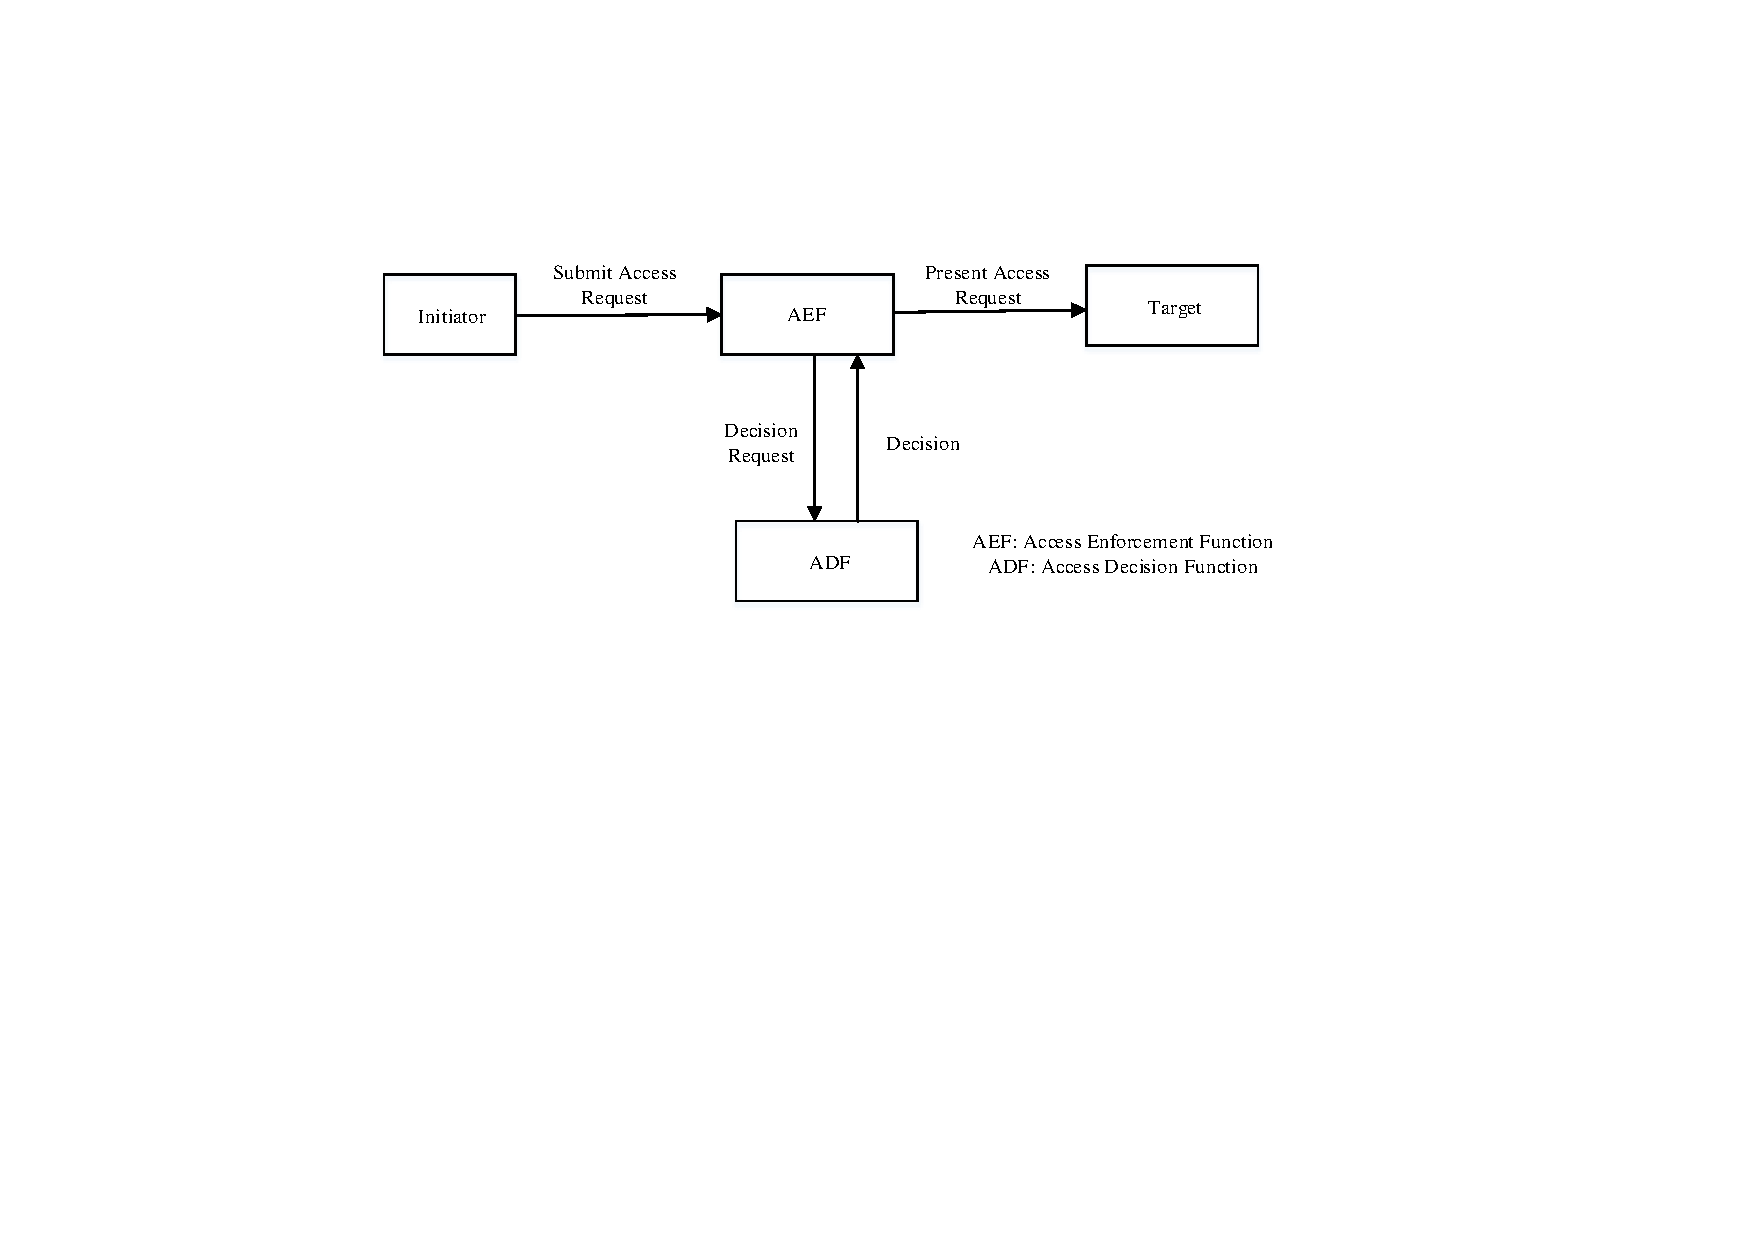
\includegraphics{12.pdf}
\newline

\textbf{Question}:

\hspace{1cm}13.Please draw the access control relationship diagram.

\textbf{Answer}:

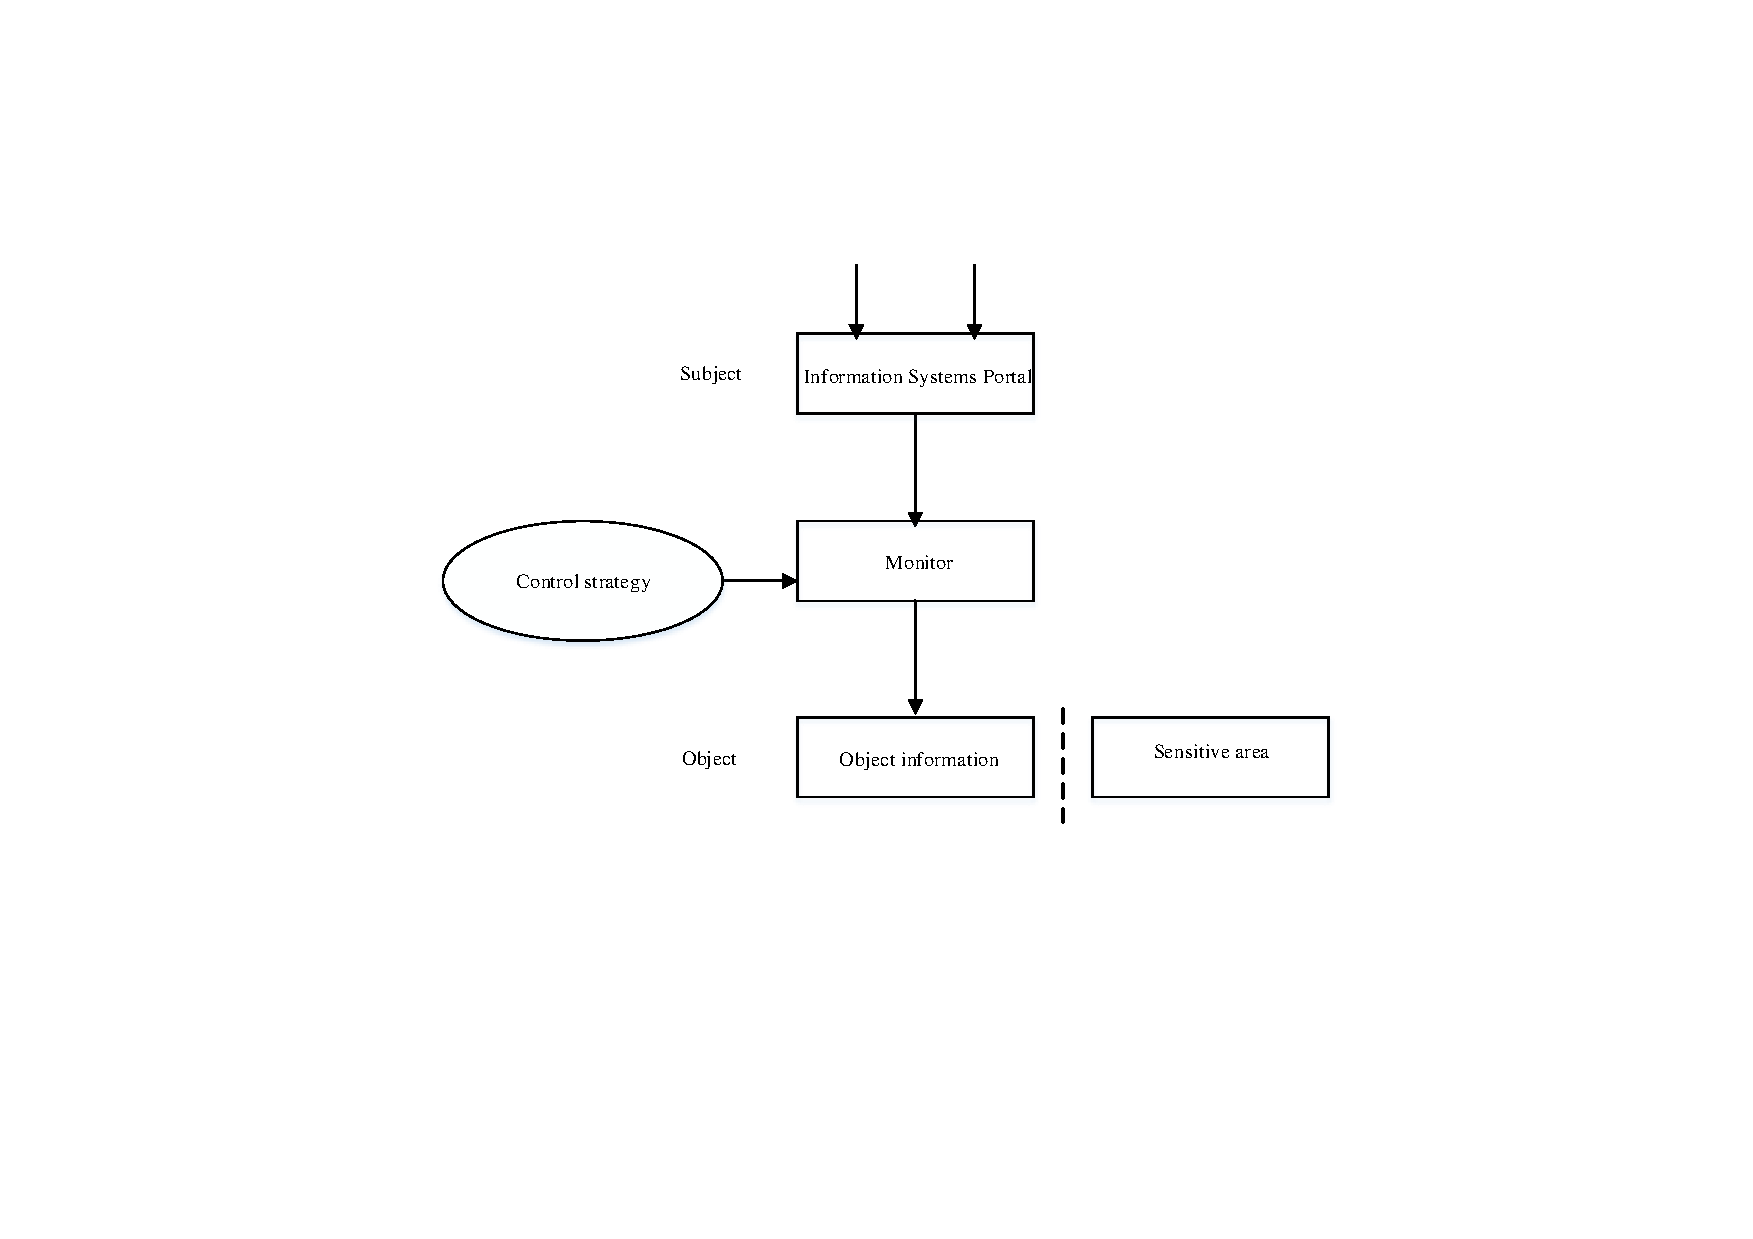
\includegraphics{20.pdf}


\section{Classic cryptography}
\label{sec:cc}

\section{Digital signature}
\label{sec:ds}

\section{Confidentiality and integrity policies}
\label{sec:cip}

\textbf{Question}:

\hspace{1cm}1.Describe the classification about Data confidentiality.

\textbf{Answer}:

\hspace{1cm}Data confidentiality is the protection of data from unauthorized disclosure.

\hspace{1cm}Connection Confidentiality: The protection of all user data on a connection.

\hspace{1cm}Connectionless Confidentiality: The protection of all user data in a single data block��

\hspace{1cm}Selective-Field Confidentiality: The confidentiality of selected fields within the user��data on a connection or in a single data block.

\hspace{1cm}Traffic-Flow Confidentiality: The protection of the information that might be
derived from observation of traffic flows.
\newline

\textbf{Question}:

\hspace{1cm}2.According to ISO7498-2, what is included in security services?

\textbf{Answer}:

\hspace{1cm}Entity Authentication

\hspace{1cm}Data Confidentiality

\hspace{1cm}Data Integrity

\hspace{1cm}Non-repudiation

\hspace{1cm}Access Control
\newline

\textbf{Question}:

\hspace{1cm}3.The SSL Record Protocol provides two services for SSL connections, what are they?

\textbf{Answer}:

\hspace{1cm}Confidentiality: The Handshake Protocol defines a shared secret key that is
used for conventional encryption of SSL payloads.

\hspace{1cm}Message Integrity: The Handshake Protocol also defines a shared secret key
that is used to form a message authentication code (MAC).
\newline

\textbf{Question}:

\hspace{1cm}4.List the threats about Integrity and Confidentiality, respectively.

\textbf{Answer}:

\hspace{1cm}Integrity:

\hspace{1cm}Modification of user data

\hspace{1cm}Trojan horse browser

\hspace{1cm}Modification of memory

\hspace{1cm}Modification of message traffic in transit

\hspace{1cm}Confidentiality:

\hspace{1cm}Eavesdropping on the net

\hspace{1cm}Theft of info from server

\hspace{1cm}Theft of data from client

\hspace{1cm}Info about network Configuration

\hspace{1cm}Info about which client talks to server
\newline

\textbf{Question}:

\hspace{1cm}5.How do access control technology reflect the confidentiality and integrity?

\textbf{Answer}:

\hspace{1cm}Read up and write down strategy, belonging to a security level can read the subject of the level and above the level of the object, you can write the level and below the level of the object, which ensures information integrity policies.

\hspace{1cm}Write up and read down strategy, belonging to a security level can write the subject of the level and above the level of the object, you can read the level and below the level of the object, which ensures information integrity policies.
\newline

\textbf{Question}:

\hspace{1cm}6.Describe the IP security services, such us RFC4301?

\textbf{Answer}:

\hspace{1cm}Access control

\hspace{1cm}Connectionless integrity

\hspace{1cm}Data origin authentication

\hspace{1cm}Rejection of replayed packet

\hspace{1cm}Confidentiality

\hspace{1cm}Limited traffic for Confidentiality
\newline

\textbf{Question}:

\hspace{1cm}7.What aspects of security do Cryptography provide for the storage and transmission of digital information?

\textbf{Answer}:

\hspace{1cm}Confidentiality: Preserving authorized restrictions on information access and disclosure, including means for protecting personal privacy and proprietary information. A loss of confidentiality is the unauthorized disclosure of information.

\hspace{1cm}Integrity: Guarding against improper information modification or destruction, including ensuring information non-repudiation and authenticity. A loss of integrity is the unauthorized modification or destruction of information.

\hspace{1cm}Identification: Once detection has been achieved, identify the specific virus that has infected a program.

\hspace{1cm}Non-repudiation: Non-repudiation prevents either sender or receiver from denying a transmitted message. Thus, when a message is sent, the receiver can prove that the alleged
sender in fact sent the message. Similarly, when a message is received, the sender can
prove that the alleged receiver in fact received the message.
\section{Key Management}
\label{sec:km}

\section{virus}
\label{sec:vs}

\section{Cryptographic Checksums}
\label{sec:checksums}


\end{document}
